% This is samplepaper.tex, a sample chapter demonstrating the
% LLNCS macro package for Springer Computer Science proceedings;
% Version 2.20 of 2017/10/04
%
\documentclass[runningheads,table]{llncs}
%
\usepackage{graphicx}

% For algorithmic attachments and graphics
\usepackage{amsmath}
\usepackage{algorithm}
\usepackage[noend]{algpseudocode}
\usepackage{subcaption}
\captionsetup{compatibility=false}

\usepackage{tikz}
\usepackage{dsfont}
\usepackage{multicol, multirow}
%\usepackage{booktabs}
\usetikzlibrary{fit,calc,automata,positioning}


% Used for displaying a sample figure. If possible, figure files should
% be included in EPS format.
%
% If you use the hyperref package, please uncomment the following line
% to display URLs in blue roman font according to Springer's eBook style:
% \renewcommand\UrlFont{\color{blue}\rmfamily}

\begin{document}
%
\title{Context-Free Path Querying by Using Kronecker Product\thanks{Supported by organization x.}}
%
%\titlerunning{Abbreviated paper title}
% If the paper title is too long for the running head, you can set
% an abbreviated paper title here
%
\author{Egor Orachev\inst{1} \and
Ilya Epelbaum\inst{1} \and
Rustam Azimov\inst{1,2} \and
Semyon Grigorev\inst{1,2}\orcidID{0000-0002-7966-0698}}
%
\authorrunning{E. Orachev et al.}
% First names are abbreviated in the running head.
% If there are more than two authors, 'et al.' is used.
%
\institute{St.Petersburg State University, 7/9 Universitetskaya nab., St. Petersburg, Russia, 199034 \\
\email{semyon.grigorev@jetbrains.com, iliyepelbaun@gmail.com, rustam.azimov19021995@gmail.com, s.v.grigoriev@spbu.ru} \and
JetBrains Research, Primorskiy prospekt 68-70, Building 1, St. Petersburg, Russia, 197374\\
\email{semyon.grigorev@jetbrains.com}}
%
\maketitle              % typeset the header of the contribution
%
\begin{abstract}
Context-free path queries (CFPQ) extend regular path queries (RPQ) and allow one to use context-free grammars as constraints for paths. Algorithms for CFPQ are actively developed, but J. Kuijpers recently concludes, that existing algorithms are not performant enough to be used in real-world applications. Thus the development of new algorithms for CFPQ is required. In this paper we provide a new CFPQ algorithm which is based on such linear algebra operations as Kronecker product and transitive closure, and handles grammars presented as recursive state machines. Thus, the proposed algorithm can be implemented by using high-performance libraries and modern parallel hardware, and avoids grammar growth, consequently, it provides the ability for queries optimization.


\keywords{Context-free path querying \and Graph database \and Context-free grammars \and CFPQ \and Kronecker product \and Recursive state machines.}
\end{abstract}
%
%
%

\section{Introduction}

Scalable high-performance graph analysis is an actual challenge.
There is a big number of ways to attack this challenge~\cite{Coimbra2021} and the first promising idea is to utilize general-purpose graphic processing units (GPGPU).
Such existing solutions, as CuSha~\cite{10.1145/2600212.2600227} and Gunrock~\cite{7967137} show that utilization of GPUs can improve the performance of graph analysis, moreover it is shown that solutions may be scaled to multi-GPU systems.
But low flexibility and high complexity of API are problems of these solutions.

The second promising thing which provides a user-friendly API for high-performance graph analysis algorithms creation is a GraphBLAS API~\cite{7761646} which provides linear algebra based building blocks to create graph analysis algorithms.
The idea of GraphBLAS is based on a well-known fact that linear algebra operations can be efficiently implemented on parallel hardware.
Along with that, a graph can be natively represented using matrices: adjacency matrix, incidence matrix, etc.
While reference CPU-based implementation of GraphBLAS, SuiteSparse:GraphBLAS~\cite{10.1145/3322125}, demonstrates good performance in real-world tasks, GPU-based implementation is challenging.

One of the challenges in this way is that real data are often sparse, thus underlying matrices and vectors are also sparse, and, as a result, classical dense data structures and respective algorithms are inefficient. 
So, it is necessary to use advanced data structures and procedures to implement sparse linear algebra, but the efficient implementation of them on GPU is hard due to the irregularity of workload and data access patterns.
Though such well-known libraries as cuSPARSE show that sparse linear algebra operations can be efficiently implemented for GPGPU, it is not so trivial to implement GraphBLAS on GPGPU. 
First of all, it requires \textit{generic} sparse linear algebra, thus it is impossible just to reuse existing libraries which are almost all specified for operations over floats.
The second problem is specific optimizations, such as masking fusion, which can not be natively implemented on top of existing kernels.
Nevertheless, there is a number of implementations of GraphBLAS on GPGPU, such as GraphBLAST~\cite{yang2019graphblast}, GBTL~\cite{7529957}, which show that GPGPUs utilization can improve the performance of GraphBLAS-based graph analysis solutions.
But these solutions are not portable because they are based on Nvidia Cuda stack.
Moreover, the scalability problem is not solved: all these solutions support only single-GPU, not multi-GPU computations.

To provide portable GPU implementation of GraphBLAS API we developed a \textit{SPLA} library\footnote{Source code available at: \url{https://github.com/JetBrains-Research/spla}}.
This library utilizes OpenCL for GPGPU computing to be portable across devices of different vendors.
Moreover, it is initially designed to utilize multiple GPGPUs to be scalable.
To sum up, the contribution of this work is the following.
\begin{itemize}
    \item Design of portable GPU GraphBLAS implementation proposed. The design involves the utilization of multiple GPUS. Additionally, the proposed design is aimed to simplify library tuning and wrappers for different high-level platforms and languages creation. 
    \item Subset of GraphBLAS API, including such operations as masking, matrix-matrix multiplication, matrix-matrix e-wise addition, is implemented. The current implementation is limited by COO and CSR matrix representation format and uses basic algorithms for some operations, but work in progress and more data formats will be supported and advanced algorithms will be implemented in the future.
    \item Preliminary evaluation on such algorithms as breadth-first search (BFS) and triangles counting (TC), and real-world graphs shows portability across different vendors and promising performance: for some problems Spla is comparable with GraphBLAST. Surprisingly, for some problems, the proposed solution on embedded Intel graphic card shows better performance than SuiteSparse:GraphBLAS on the respective CPU. At the same time, the evaluation shows that further optimization is required.
\end{itemize} 
\section{Recursive State Machines}
\label{section:rsm}

In this section, we introduce recursive state machines (RSM)~\cite{rsm:analysis:10.1007/3-540-44585-4_18}.
This kind of computational machine extends the definition of finite state machines and increases the computational capabilities of this formalism.

A recursive state machine $R$ over a finite alphabet $\Sigma$ is defined as a tuple of elements $(M,m,\{C_i\}_{i \in M})$, where:

\begin{itemize}
    \item $M$ is a finite set of labels of boxes.
    \item $m \in M$ is an initial box label.
    \item Set of \textit{component state machines} or \textit{boxes},
          where $C_i=(\Sigma \cup M, Q_i,q_i^0,F_i,\delta_i)$:
    \begin{itemize}
        \item $\Sigma \cup M$ is a set of symbols, $\Sigma \cap M = \emptyset$
        \item $Q_i$ is a finite set of states,
              where $Q_i \cap Q_j = \emptyset, \forall i \neq j$
        \item $q_i^0$ is an initial state for the component state machine $C_i$
        \item $F_i$ is a set of final states for $C_i$, where $F_i \subseteq Q_i$
        \item $\delta_i$ is a transition function for $C_i$,
              where $\delta_i: Q_i \times (\Sigma \cup M)
              \to Q_i$
    \end{itemize}
\end{itemize}

RSM behaves as a set of finite state machines (or FSM).
Each FSM is called a \textit{box} or a \textit{component state machine}~\cite{rsm:analysis:10.1007/3-540-44585-4_18}.
A box works almost the same as a classical FSM, but it also handles additional \textit{recursive calls} and employs an implicit \textit{call stack} to \textit{call} one component from another and then return execution flow back.

The execution of an RSM could be defined as a sequence of the configuration transitions, which are done on input symbols reading. 
The pair $(q_i,S)$, where $q_i$ is current state for box $C_i$ and $S$ is stack of \textit{return states}, describes execution configurations. 

The RSM execution starts form configuration $(q_m^0, \langle\rangle)$. 
The following list of rules defines the machine transition from configuration $(q_i,S)$ to $(q',S')$ on some input symbol $a$ from the input sequence, which is read as usual for FSA:

\begin{itemize}
    \item $q' \gets q_i^t, S' \gets S$, where $q_i^t = \delta_i (q_i^k, a), q_i^k = q$
    \item $q' \gets q_j^0, S' \gets q_i^t \circ S$, where $q_i^t = \delta_i (q_i^k, j),  q_i^k = q, j \in M$
    \item $q' \gets q_i^t, S' \gets S_{tail}$, where $S = q_i^t \circ S_{tail}, q_j^k = q, q_j^k \in F_j$
\end{itemize}

Some input sequence of the symbols $a_1 ... a_n$, which forms some input word, accepted, if machine reaches configuration $(q,\langle\rangle)$, where $q \in F_m$. It is also worth noting that the  RSM makes not deterministic transitions, without reading the input character when it \textit{calls} some component or makes a \textit{return}.

%The execution of RSM $R$ is a sequance of transitions between configurations of form $(q,S)$, where $S$ is global stack of \textit{return states} from $\bigcup_{i \in M}Q_i$ such as $S=\langle ...q_r \rangle$, and $q \in \bigcup_{i \in M}Q_i$ is a current state of the machine. The execution starts from box $m$ initial state $q_m^0$ and empty stack as follows $(q_m^0,\langle \rangle)$. Transitions for a given global machine state $(q,S)$ to some new state $(q',S')$ are defined as follows:

%\begin{itemize}
%    \item $q':=q_b', S':=S$,
%    where $\delta_b (q_b,s) \to q_b', s \in \Sigma,
%    q=q_b, S = \langle ...q_r \rangle$
%    \item $q':=q_t^0, S':=\langle ...q_r,q_b'\rangle$,
%    where $\delta_b (q_b,t) \to q_b', t \in M, q=q_b, S = \langle ...q_r \rangle$
%    \item $q':=q_b', S':=\langle ...q_r \rangle$,
%    where $q=q_t^i, q_t^i \in F_t, S=\langle ...q_r,q_b' \rangle$
%\end{itemize}

According to~\cite{rsm:analysis:10.1007/3-540-44585-4_18}, recursive state machines are equivalent to pushdown systems.
Since pushdown systems are capable of accepting context-free languages~\cite{automata:theory:10.5555/1177300}, it is clear that RSMs are equivalent to context-free languages.
Thus RSMs suit to encode query grammars.
Any CFG can be easily converted to an RSM with one box per nonterminal.
The box which corresponds to a nonterminal $A$ is constructed using the right-hand side of each rule for $A$.
An example of such RSM $R$ constructed for the grammar $G$ with rules $S \to a S b \mid a b$ is provided in figure~\ref{example:automata}.

%We escape detailed discussion of the conversion of a context free grammar $G$ to a RSM $R$. In the basic case, an algorithm for constructing such RSM could be composed from several stages, where each stage involves building of finite state machine for each non-terminal $N$ from grammar $G$.

Since $R$ is a set of FSMs, it is useful to represent $R$ as an adjacency matrix for the graph where vertices are states from $\bigcup_{i \in M}Q_i$ and edges are transitions between $q_i^a$ and $q_i^b$ with label $l \in \Sigma \cup M$, if $\delta_i (q_i^a, l) = q_i^b$.
An example of such adjacency matrix $M_R$ for the machine $R$ is provided in section~\ref{example:section}.

\begin{figure}[h]
    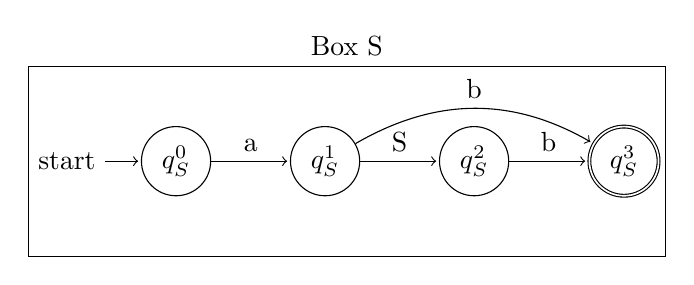
\begin{tikzpicture}[shorten >=1pt,auto]
        \node[state, initial] (q_0)   {$q_S^0$};
        \node[state] (q_1) [right=of q_0] {$q_S^1$};
        \node[state] (q_2) [right=of q_1] {$q_S^2$};
        \node[state, accepting] (q_3) [right=of q_2] {$q_S^3$};
        \path[->]
            (q_0) edge node {a} (q_1)
            (q_1) edge node {S} (q_2)
            (q_2) edge node {b} (q_3)
            (q_1) edge [bend left, above]  node {b} (q_3);
        \node[draw=black, fit= (q_0) (q_1) (q_2) (q_3), xshift=-4.5ex,inner sep=0.75cm, label=Box S] {};
    \end{tikzpicture}
    \centering
    \caption{The recursive state machine $R$ for grammar $G$}
    \label{example:automata}
\end{figure}


\section{Kronecker Product Based CFPQ Algorithm}

The idea of the algorithm is based on generalisation of the finite-state machine intersection for a recursive automata, created from input grammar, and an input graph. The result of the intersection is evaluated as a Kronecker product of the corresponding adjacency matrices for automata and graph. To solve reachability problem it is enough to represent intersection result as a Boolean matrix, what simplifies algorithm implementation and allows to express it in terms of basic matrix operations. Listing~\ref{tensor:cfpq}. shows main steps of the solution.

As an input algorithm accepts context-free grammar $G=(\Sigma,N,P$) and graph $\mathcal{G}=(V,E,L)$. All sets in the grammar and graph are supposed to be of finite size. Recursive automata $R$ is created from $G$. The process of the creation is out of the scope of this article. $M_1$ and $M_2$ are the adjacency matrices for automata $R$ and graph $\mathcal{G}$ correspondingly. Cell values of this matrices could be represented as sets of elements from $L \cup N \cup \Sigma$.

Then the $\varepsilon$ symbol is explicitly added for matrices $M_1$ and $M_2$. For each state of the $R$ algorithm adds transitions from state $i$ to state $i$ via $\varepsilon$ if $i$ is initial and final state for some non-terminal. This info is queried via $getNonterminals()$ function call. Also for each vertex $i$ of the graph $\mathcal{G}$ the edge from $i$ to $i$ with label $\varepsilon$ is added. Here the rule is implied: each vertex of the graph $\mathcal{G}$ is reachable by itself through $\varepsilon$-transition. 

The algorithm is executed while matrix $M_2$ is changing. For each iteration Kronecker product of matrices $M_1$ and $M_2$ is evaluated. The result is saved in $M_3$ as a Boolean matrix. For given $M_3$ evaluated $C_3$ matrix via $transitiveClosure()$ function call. The $M_3$ could be interpreted as an adjacency matrix for an oriented graph without labels, used to evaluate transitive closure in terms of classical graph definition of this operation. Then the algorithm iterates over cells of the $C_3$. For pair of indices $(i,j)$ computes $s$ and $f$ - initial and final states in recursive automata $R$ which relate to the concrete $C_3[i,j]$ of the tensor matrix. Function $hasPathForNonterminals()$ checks whether for given $s$ and $f$ states automata has at least one non-terminal path. If the conditional statement is $true$ then algorithm adds non-terminals of that path via $getNonterminals()$ to the concrete cell of the adjacency matrix $M_2$ of the graph.

As an result the algorithm returns updated matrix $M_2$ which contains initial graph $\mathcal{G}$ data and non-terminals from $N$. If a cell $M_2[i,j]$ for any valid indices $i$ and $j$ contains symbol $S \in N$, therefore, vertex $j$ is reachable from vertex $i$ in grammar $G$ for non-terminal $S$.

\begin{algorithm}[h]
\floatname{algorithm}{Listing}
\begin{algorithmic}[1]
\caption{Kronecker product based CFPQ}
\label{tensor:cfpq}
\Function{contextFreePathQuerying}{G, $\mathcal{G}$}
    % Input data preparation
    \State{$R \gets$ Recursive automata for $G$}
    \State{$M_1 \gets$ Adjacency matrix for $R$}
    \State{$M_2 \gets$ Adjacency matrix for $\mathcal{G}$}
    % Eps-transition handling for graph
    \For{$i \in 0..dim(M_1)-1$} 
        \If{$|\textit{getNonterminals}(R,i,i)| > 0$}
            \Comment{Has at least one non-terminal}
            \State{$M_2[i,i] \gets M_2[i,i] \cup \{ \varepsilon \}$}
        \EndIf
    \EndFor
    % Eps-transition handling for graph
    \For{$i \in 0..dim(M_2)-1$} 
        \State{$M_3[i,i] \gets M_3[i,i] \cup \{ \varepsilon \}$}
    \EndFor
    \While{Matrix $M_2$ is changing}
        \State{$M_3 \gets M_1 \otimes M_2$}
        \Comment{Evaluate tensor product}
        \State{$C_3 \gets \textit{transitiveClosure}(M_3)$}
        \State{$n \gets$ dim($M_3)$}
        \Comment{Matrix $M_3$ size = $n \times n$}
        % Add non-terminals (possibly new)
        \For{$i \in 0..n-1$}
           \For{$j \in 0..n-1$}
                \If{$C_3[i,j]$}
                    \State{$s, f \gets \textit{getStates}(C_3,i,j)$}
                    \If{$\textit{hasPathForNonterminals}(R,s,f)$}
                        \State{$x, y \gets \textit{getCoordinates}(C_3,i,j)$}
                        \State{$M_2[x,y] \gets M_2[x,y] \cup \textit{getNonterminals}(R,s,f)$}
                    \EndIf
                \EndIf
           \EndFor
        \EndFor
    \EndWhile
\State \Return $M_2$
\EndFunction
\end{algorithmic}
\end{algorithm}

Since the Kronecker product evaluated in the fixed order, such as $M_1 \otimes M_2$, the functions $getStates$ and $getCoordinates$ could be implemented as shown in Listing~\ref{tensor:cfpq:help}. This implementation appeals to the blocked structure of the matrix $C_3$, where each block corresponds to some automata and graph edge.

\begin{algorithm}[h]
\floatname{algorithm}{Listing}
\begin{algorithmic}[1]
\caption{Help functions for Kronecker product based CFPQ}
\label{tensor:cfpq:help}
\Function{getStates}{$C, i, j$}
    \State{$r \gets dim(M_1)$}
    \Comment{$M_1$ is adjacency matrix for automata $R$}
    \State \Return{$\left\lfloor{i / r}\right\rfloor, \left\lfloor{j / r}\right\rfloor$}
\EndFunction
\Function{getCoordinates}{$C, i, j$}
    \State{$n \gets dim(M_2)$}
    \Comment{$M_2$ is adjacency matrix for graph $\mathcal{G}$}
    \State \Return{$i \bmod n, j \bmod n$}
\EndFunction
\end{algorithmic}
\end{algorithm}

The proposed algorithm terminates in finite number of steps. Since functions, used in the algorithm, terminate in finite number of steps, it is enough to proof that the $while$ loop takes finite number of iterations. The matrix $M_2$ is updated only by possible addition of the new non-terminals in the line \textbf{20}. The number of elements in the cell of matrix $M_2$ only grows and cannot exceed $|L \cup N \cup \Sigma|$. Therefore, the $while$ loop terminates in finite number of iterations, which no more than $|L \cup N \cup \Sigma| * |V|^2$ in case when only 1 symbol is added for only one vertex per iteration.

\subsection{Example}

This section is intended to provide step-by-step demonstration of the proposed algorithm. As an example consider the following query, theoretical worst case for CFPQ time complexity, proposed by Hellings~\cite{Hellings}: graph $\mathcal{G}$ presented in Figure~\ref{input:graph} and  context-free grammar $G=(\Sigma,N,P)$ for a language $\{a^n b^n | n \geq 1\}$ where:

\begin{itemize}
    \item Set of terminals $\Sigma = \{a, b\}$.
    \item Set of non-terminals $V = \{ S \}$.
    \item Set of production rules $P = \{ S \to a S b, S \to a b\}$.
\end{itemize}

Since the proposed algorithm processes grammar in form of recursive automata, we first provide automata $R$ in Figure~\ref{input:automata}. The initial state of the automata is $(0)$, the final state is $(3)$. The notation $\{S\}$ denotes here that non-terminal $S$ could be derived in automata path from vertex $(0)$ to $(3)$.

\begin{figure}[h]
     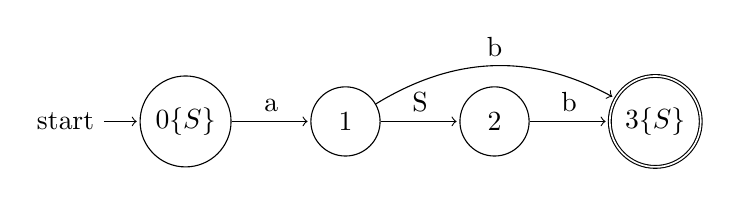
\begin{tikzpicture}[shorten >=1pt,auto]
           \node[state, initial] (q_0)   {$0 \{S\}$};
           \node[state] (q_1) [right=of q_0] {$1$};
           \node[state] (q_2) [right=of q_1] {$2$};
           \node[state, accepting] (q_3) [right=of q_2] {$3\{S\}$};
            \path[->]
            (q_0) edge node {a} (q_1)
            (q_1) edge node {S} (q_2)
            (q_2) edge node {b} (q_3)
            (q_1) edge [bend left, above]  node {b} (q_3);
    \end{tikzpicture}
    \centering
    \caption{The recursive automata $R$ of grammar $G$ for example query}
    \label{input:automata}
\end{figure}

\begin{figure}[h]
        \centering
        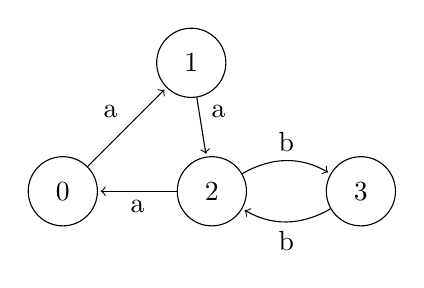
\begin{tikzpicture}[shorten >=1pt,auto]
           \node[state] (q_0)                      {$0$};
           \node[state] (q_1) [above right=of q_0] {$1$};
           \node[state] (q_2) [right=of q_0]       {$2$};
           \node[state] (q_3) [right=of q_2]       {$3$};
            \path[->]
            (q_0) edge  node {a} (q_1)
            (q_1) edge  node {a} (q_2)
            (q_2) edge  node {a} (q_0)
            (q_2) edge[bend left, above]  node {b} (q_3)
            (q_3) edge[bend left, below]  node {b} (q_2);
        \end{tikzpicture}
        \caption{The input graph $\mathcal{G}$ for example query}
        \label{input:graph}
\end{figure}

Adjacency matrices $M_1$ and $M_2$ for automata $R$ and graph $\mathcal{G}$ respectively are initialised as follows:
    $$
    M_1 =
    \begin{pmatrix}
    . & . & \{a\} & .     \\
    . & . & \{S\} & \{b\} \\
    . & . & . & \{b\}     \\
    . & . & . & .
    \end{pmatrix}
    ,~~~~~
    M_2^0 =
    \begin{pmatrix}
    . & \{a\} & . & .     \\
    . & . & \{a\} & .     \\
    \{a\} & . & . & \{b\} \\
    . & . & \{b\} & .
    \end{pmatrix}.
    $$

After all the data is initialised in lines \textbf{2--4}, the algorithm handles $\varepsilon$-case. Because automata $R$ does not have $\varepsilon$-transitions and $\varepsilon$-word is not included in grammar $G$ language lines \textbf{5-9} of the algorithm do not affect on the input data.

Then the algorithm enters while loop and iterates as long as matrix $M_2$ is changing. We provide step-by-step evaluation of matrices $M_3$, $C_3$ and updating of matrix $M_2$. All the matrices are denoted with upper index of the current loop iteration. The first loop iteration is indexed as 1.

For the first while loop iteration the tensor product $M_3^1 = M_1 \otimes M_2^0$ and transitive closure $C_3^1$ are evaluated as follows:

%\begin{figure}
    {\renewcommand{\arraystretch}{0.6}
    %\centering
    $$
    M_3^1 =
    \left(
    \begin{array}{c c c c | c c c c | c c c c | c c c c }
    . & . & . & .  &  . & 1 & . & .  &  . & . & . & .  &  . & . & . & .   \\
    . & . & . & .  &  . & . & 1 & .  &  . & . & . & .  &  . & . & . & .   \\
    . & . & . & .  &  1 & . & . & .  &  . & . & . & .  &  . & . & . & .   \\
    . & . & . & .  &  . & . & . & .  &  . & . & . & .  &  . & . & . & .   \\
    \hline
    . & . & . & .  &  . & . & . & .  &  . & . & . & .  &  . & . & . & .   \\
    . & . & . & .  &  . & . & . & .  &  . & . & . & .  &  . & . & . & .   \\
    . & . & . & .  &  . & . & . & .  &  . & . & . & .  &  . & . & . & 1   \\
    . & . & . & .  &  . & . & . & .  &  . & . & . & .  &  . & . & 1 & .   \\
    \hline
    . & . & . & .  &  . & . & . & .  &  . & . & . & .  &  . & . & . & .   \\
    . & . & . & .  &  . & . & . & .  &  . & . & . & .  &  . & . & . & .   \\
    . & . & . & .  &  . & . & . & .  &  . & . & . & .  &  . & . & . & 1   \\
    . & . & . & .  &  . & . & . & .  &  . & . & . & .  &  . & . & 1 & . \\
    \hline
    . & . & . & .  &  . & . & . & .  &  . & . & . & .  &  . & . & . & .   \\
    . & . & . & .  &  . & . & . & .  &  . & . & . & .  &  . & . & . & .   \\
    . & . & . & .  &  . & . & . & .  &  . & . & . & .  &  . & . & . & .   \\
    . & . & . & .  &  . & . & . & .  &  . & . & . & .  &  . & . & . & .
    \end{array}
    \right)
    ,~~~~~~
    C_3^1 =
    \left(
    \begin{array}{c c c c | c c c c | c c c c | c c c c }
    . & . & . & .  &  . & 1 & . & .  &  . & . & . & .  &  . & . & . & . \\
    . & . & . & .  &  . & . & 1 & .  &  . & . & . & .  &  . & . & . & \cellcolor{lightgray}\textbf{1} \\
    . & . & . & .  &  1 & . & . & .  &  . & . & . & .  &  . & . & . & . \\
    . & . & . & .  &  . & . & . & .  &  . & . & . & .  &  . & . & . & . \\
    \hline
    . & . & . & .  &  . & . & . & .  &  . & . & . & .  &  . & . & . & . \\
    . & . & . & .  &  . & . & . & .  &  . & . & . & .  &  . & . & . & . \\
    . & . & . & .  &  . & . & . & .  &  . & . & . & .  &  . & . & . & 1 \\
    . & . & . & .  &  . & . & . & .  &  . & . & . & .  &  . & . & 1 & . \\
    \hline
    . & . & . & .  &  . & . & . & .  &  . & . & . & .  &  . & . & . & . \\
    . & . & . & .  &  . & . & . & .  &  . & . & . & .  &  . & . & . & . \\
    . & . & . & .  &  . & . & . & .  &  . & . & . & .  &  . & . & . & 1 \\
    . & . & . & .  &  . & . & . & .  &  . & . & . & .  &  . & . & 1 & . \\
    \hline
    . & . & . & .  &  . & . & . & .  &  . & . & . & .  &  . & . & . & . \\
    . & . & . & .  &  . & . & . & .  &  . & . & . & .  &  . & . & . & . \\
    . & . & . & .  &  . & . & . & .  &  . & . & . & .  &  . & . & . & . \\
    . & . & . & .  &  . & . & . & .  &  . & . & . & .  &  . & . & . & .
    \end{array}
    \right).
    $$
    }
    %\caption{The first iteration tensor product and transitive closure evaluation for example query}
    %\label{example:iteration1eval}
%\end{figure}

Note here that the dimension $n$ of the matrix $M_3$ equals 16, and this value is constant in time of the algorithm execution.

After the transitive closure evaluation matrix $C_3^1$ cell $(1,15)$ contains non-zero value. It means that vertex with index $15$ is accessible from vertex with index $1$ in a graph, represented by adjacency matrix $M_3^1$.

Then the algorithm lines \textbf{14--20} are executed. In that section algorithm adds non-terminals to the graph matrix $M_2^1$. Because this step is additive we are only interested in newly appeared values in matrix $C_3^1$ such as value $C_3^1[1,15]$.

For the value $C_3^1[1,15]$:
\begin{itemize}
    \item Indices of the automata vertices $s = 0$ and $f = 3$, because value $C_3^1[1,15]$ located in upper right matrix block $(0,3)$.
    \item Indices of the graph vertices $x = 1$ and $y = 3$ are evaluated as
    value $C_3^1[1,15]$ indices relatively to its block $(0,3)$.
    \item Function call $hasPathForNonterminals()$ returns \textbf{true} since the automata $R$ has path for non-terminal $S$ from vertex $0$ to $3$.
    \item Function call $getNonterminals()$ returns $\{S\}$ since this is the only non-terminal which could be derived in path from vertex $0$ to $3$.
\end{itemize}{}

\begin{figure}[h]
    \begin{subfigure}[]{0.5\textwidth}
    \centering
    $$
    M_2^1 =
    \begin{pmatrix}
    . & \{a\} & . & .     \\
    . & . & \{a\} & \{S\} \\
    \{a\} & . & . & \{b\} \\
    . & . & \{b\} & .
    \end{pmatrix}
    $$
    \end{subfigure}
    \begin{subfigure}[]{0.4\textwidth}
    \centering
    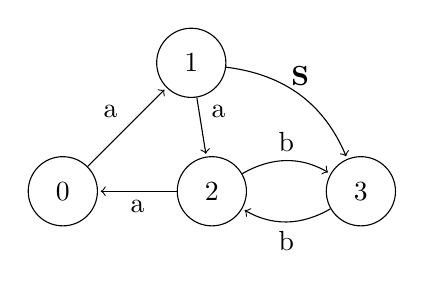
\begin{tikzpicture}[shorten >=1pt,auto]
           \node[state] (q_0)                      {$0$};
           \node[state] (q_1) [above right=of q_0] {$1$};
           \node[state] (q_2) [right=of q_0]       {$2$};
           \node[state] (q_3) [right=of q_2]       {$3$};
            \path[->]
            (q_0) edge  node {a} (q_1)
            (q_1) edge  node {a} (q_2)
            (q_1) edge[bend left, above]  node {\textbf{S}} (q_3)
            (q_2) edge  node {a} (q_0)
            (q_2) edge[bend left, above]  node {b} (q_3)
            (q_3) edge[bend left, below]  node {b} (q_2);
    \end{tikzpicture}
    \end{subfigure}
    \caption{The updated matrix $M_2^1$ and graph $\mathcal{G}$ after first loop iteration for example query}
    \label{example:iteration1res}
\end{figure}

After the first loop iteration matrix symbol $S$ is added to the cell $M_2^1[1,3]$. It is relevant data, because initial graph has path $1 \to 2 \to 3$ which could be derived for $S$. The updated matrix and graph are depicted in Figure~\ref{example:iteration1res}.

For the second loop iteration matrices $M_3^2$ and $C_3^2$ are evaluated as listed in Figure~\ref{example:iteration2eval}. For this iteration in the matrix $C_3^2$ appeared new non-zero values in cells with indices $[0,11]$, $[0,14]$ and $[5,14]$. Because only the cell value with index $[0,14]$ corresponds to the automata path with not empty non-terminal set $\{S\}$ its data affects adjacency matrix $M_2$. The updated matrix and graph $\mathcal{G}$ are depicted in Figure~\ref{example:iteration2res}.

\begin{figure}
    \renewcommand{\arraystretch}{0.6}
    \centering
    $$
    M_3^2 =
    \left(
    \begin{array}{c c c c | c c c c | c c c c | c c c c }
    . & . & . & .  &  . & 1 & . & .  &  . & . & . & .  &  . & . & . & .   \\
    . & . & . & .  &  . & . & 1 & .  &  . & . & . & .  &  . & . & . & .   \\
    . & . & . & .  &  1 & . & . & .  &  . & . & . & .  &  . & . & . & .   \\
    . & . & . & .  &  . & . & . & .  &  . & . & . & .  &  . & . & . & .   \\
    \hline
    . & . & . & .  &  . & . & . & .  &  . & . & . & .           &  . & . & . & .   \\
    . & . & . & .  &  . & . & . & .  &  . & . & . & \textbf{1}  &  . & . & . & .   \\
    . & . & . & .  &  . & . & . & .  &  . & . & . & .           &  . & . & . & 1 \\
    . & . & . & .  &  . & . & . & .  &  . & . & . & .           &  . & . & 1 & . \\
    \hline
    . & . & . & .  &  . & . & . & .  &  . & . & . & .  &  . & . & . & .   \\
    . & . & . & .  &  . & . & . & .  &  . & . & . & .  &  . & . & . & .   \\
    . & . & . & .  &  . & . & . & .  &  . & . & . & .  &  . & . & . & 1 \\
    . & . & . & .  &  . & . & . & .  &  . & . & . & .  &  . & . & 1 & . \\
    \hline
    . & . & . & .  &  . & . & . & .  &  . & . & . & .  &  . & . & . & .   \\
    . & . & . & .  &  . & . & . & .  &  . & . & . & .  &  . & . & . & .   \\
    . & . & . & .  &  . & . & . & .  &  . & . & . & .  &  . & . & . & .   \\
    . & . & . & .  &  . & . & . & .  &  . & . & . & .  &  . & . & . & .
    \end{array}
    \right)
    C_3^2 =
    \left(
    \begin{array}{c c c c | c c c c | c c c c | c c c c }
    . & . & . & .  &  . & 1 & . & .  &  . & . & . & \textbf{1}  &  . & . & \textbf{1} & . \\
    . & . & . & .  &  . & . & 1 & .  &  . & . & . & .  &  . & . & . & 1 \\
    . & . & . & .  &  1 & . & . & .  &  . & . & . & .  &  . & . & . & . \\
    . & . & . & .  &  . & . & . & .  &  . & . & . & .  &  . & . & . & . \\
    \hline
    . & . & . & .  &  . & . & . & .  &  . & . & . & .  &  . & . & . & . \\
    . & . & . & .  &  . & . & . & .  &  . & . & . & 1  &  . & . & \textbf{1} & . \\
    . & . & . & .  &  . & . & . & .  &  . & . & . & .  &  . & . & . & 1 \\
    . & . & . & .  &  . & . & . & .  &  . & . & . & .  &  . & . & 1 & . \\
    \hline
    . & . & . & .  &  . & . & . & .  &  . & . & . & .  &  . & . & . & . \\
    . & . & . & .  &  . & . & . & .  &  . & . & . & .  &  . & . & . & . \\
    . & . & . & .  &  . & . & . & .  &  . & . & . & .  &  . & . & . & 1 \\
    . & . & . & .  &  . & . & . & .  &  . & . & . & .  &  . & . & 1 & . \\
    \hline
    . & . & . & .  &  . & . & . & .  &  . & . & . & .  &  . & . & . & . \\
    . & . & . & .  &  . & . & . & .  &  . & . & . & .  &  . & . & . & . \\
    . & . & . & .  &  . & . & . & .  &  . & . & . & .  &  . & . & . & . \\
    . & . & . & .  &  . & . & . & .  &  . & . & . & .  &  . & . & . & .
    \end{array}
    \right)
    $$
    \caption{The second iteration tensor product and transitive closure evaluation for example query}
    \label{example:iteration2eval}
\end{figure}

\begin{figure}
    \begin{subfigure}[]{0.5\textwidth}
    \centering
    $$
    M_2^2 =
    \begin{pmatrix}
    .     & \{a\} & \{S\} & .     \\
    .     & .     & \{a\} & \{S\} \\
    \{a\} & .     & .     & \{b\} \\
    .     & .     & \{b\} & .
    \end{pmatrix}
    $$
    \end{subfigure}
    \begin{subfigure}[]{0.4\textwidth}
    \centering
    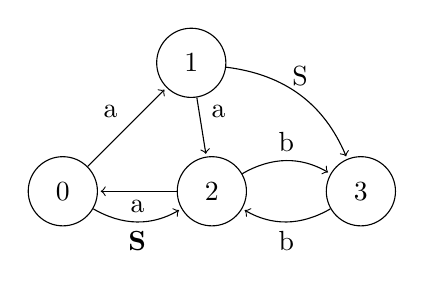
\begin{tikzpicture}[shorten >=1pt,auto]
           \node[state] (q_0)                      {$0$};
           \node[state] (q_1) [above right=of q_0] {$1$};
           \node[state] (q_2) [right=of q_0]       {$2$};
           \node[state] (q_3) [right=of q_2]       {$3$};
            \path[->]
            (q_0) edge  node {a} (q_1)
            (q_1) edge  node {a} (q_2)
            (q_1) edge[bend left, above]  node {S} (q_3)
            (q_2) edge  node {a} (q_0)
            (q_0) edge[bend right, below]  node {\textbf{S}} (q_2)
            (q_2) edge[bend left, above]  node {b} (q_3)
            (q_3) edge[bend left, below]  node {b} (q_2);
    \end{tikzpicture}
    \end{subfigure}
    \caption{The updated matrix $M_2^2$ and graph $\mathcal{G}$ after second loop iteration for example query}
    \label{example:iteration2res}
\end{figure}

The remaining matrices $C_3$ and $M_2$ for the algorithm main loop execution are listed in the Figure~\ref{example:iteration3to6eval} and Figure~\ref{example:iteration3to6res} correspondingly. For the sake of simplicity evaluated matrices $M_3$ are not included because its computation is a straightforward process. The last loop iteration is $7$. Although the matrix $M_2^6$ is updated with new non-terminal $S$ for the cell $[2,2]$ after transitive closure evaluation the new values to the matrix $M_2$ is not added. Therefore matrix $M_2$ has stopped changing and the algorithm is successfully finished.

For the example query algorithm takes $7$ iterations for the $while-loop$. The updated graph $\mathcal{G}$ is depicted in the Figure~\ref{example:result}.

\begin{figure}
    \renewcommand{\arraystretch}{0.6}
    \centering
    $$
    C_3^3 =
    \left(
    \begin{array}{c c c c | c c c c | c c c c | c c c c }
    . & . & . & .  &  . & 1 & . & .  &  . & . & . & 1  &  . & . & 1 & . \\
    . & . & . & .  &  . & . & 1 & .  &  . & . & . & .  &  . & . & . & 1 \\
    . & . & . & .  &  1 & . & . & .  &  . & . & \cellcolor{lightgray}\textbf{1} & .  &  . & . & . & \cellcolor{lightgray}\textbf{1} \\
    . & . & . & .  &  . & . & . & .  &  . & . & . & .  &  . & . & . & . \\
    \hline
    . & . & . & .  &  . & . & . & .  &  . & . & 1 & .  &  . & . & . & \textbf{1} \\
    . & . & . & .  &  . & . & . & .  &  . & . & . & 1  &  . & . & 1 & . \\
    . & . & . & .  &  . & . & . & .  &  . & . & . & .  &  . & . & . & 1 \\
    . & . & . & .  &  . & . & . & .  &  . & . & . & .  &  . & . & 1 & . \\
    \hline
    . & . & . & .  &  . & . & . & .  &  . & . & . & .  &  . & . & . & . \\
    . & . & . & .  &  . & . & . & .  &  . & . & . & .  &  . & . & . & . \\
    . & . & . & .  &  . & . & . & .  &  . & . & . & .  &  . & . & . & 1 \\
    . & . & . & .  &  . & . & . & .  &  . & . & . & .  &  . & . & 1 & . \\
    \hline
    . & . & . & .  &  . & . & . & .  &  . & . & . & .  &  . & . & . & . \\
    . & . & . & .  &  . & . & . & .  &  . & . & . & .  &  . & . & . & . \\
    . & . & . & .  &  . & . & . & .  &  . & . & . & .  &  . & . & . & . \\
    . & . & . & .  &  . & . & . & .  &  . & . & . & .  &  . & . & . & .
    \end{array}
    \right)
    C_3^4 =
    \left(
    \begin{array}{c c c c | c c c c | c c c c | c c c c }
    . & . & . & .  &  . & 1 & . & .  &  . & . & . & 1  &  . & . & 1 & . \\
    . & . & . & .  &  . & . & 1 & .  &  . & . & . & \textbf{1}  &  . & . & \textbf{1} & 1 \\
    . & . & . & .  &  1 & . & . & .  &  . & . & 1 & .  &  . & . & . & 1 \\
    . & . & . & .  &  . & . & . & .  &  . & . & . & .  &  . & . & . & . \\
    \hline
    . & . & . & .  &  . & . & . & .  &  . & . & 1 & .  &  . & . & . & 1 \\
    . & . & . & .  &  . & . & . & .  &  . & . & . & 1  &  . & . & 1 & . \\
    . & . & . & .  &  . & . & . & .  &  . & . & . & 1  &  . & . & \textbf{1} & 1 \\
    . & . & . & .  &  . & . & . & .  &  . & . & . & .  &  . & . & 1 & . \\
    \hline
    . & . & . & .  &  . & . & . & .  &  . & . & . & .  &  . & . & . & . \\
    . & . & . & .  &  . & . & . & .  &  . & . & . & .  &  . & . & . & . \\
    . & . & . & .  &  . & . & . & .  &  . & . & . & .  &  . & . & . & 1 \\
    . & . & . & .  &  . & . & . & .  &  . & . & . & .  &  . & . & 1 & . \\
    \hline
    . & . & . & .  &  . & . & . & .  &  . & . & . & .  &  . & . & . & . \\
    . & . & . & .  &  . & . & . & .  &  . & . & . & .  &  . & . & . & . \\
    . & . & . & .  &  . & . & . & .  &  . & . & . & .  &  . & . & . & . \\
    . & . & . & .  &  . & . & . & .  &  . & . & . & .  &  . & . & . & .
    \end{array}
    \right)
    $$
    $$
    C_3^5 =
    \left(
    \begin{array}{c c c c | c c c c | c c c c | c c c c }
    . & . & . & .  &  . & 1 & . & .  &  . & . & \textbf{1} & 1  &  . & . & 1 & \textbf{1} \\
    . & . & . & .  &  . & . & 1 & .  &  . & . & . & 1  &  . & . & 1 & 1 \\
    . & . & . & .  &  1 & . & . & .  &  . & . & 1 & .  &  . & . & . & 1 \\
    . & . & . & .  &  . & . & . & .  &  . & . & . & .  &  . & . & . & . \\
    \hline
    . & . & . & .  &  . & . & . & .  &  . & . & 1 & .  &  . & . & . & 1 \\
    . & . & . & .  &  . & . & . & .  &  . & . & 1 & 1  &  . & . & 1 & \textbf{1} \\
    . & . & . & .  &  . & . & . & .  &  . & . & . & 1  &  . & . & 1 & 1 \\
    . & . & . & .  &  . & . & . & .  &  . & . & . & .  &  . & . & 1 & . \\
    \hline
    . & . & . & .  &  . & . & . & .  &  . & . & . & .  &  . & . & . & . \\
    . & . & . & .  &  . & . & . & .  &  . & . & . & .  &  . & . & . & . \\
    . & . & . & .  &  . & . & . & .  &  . & . & . & .  &  . & . & . & 1 \\
    . & . & . & .  &  . & . & . & .  &  . & . & . & .  &  . & . & 1 & . \\
    \hline
    . & . & . & .  &  . & . & . & .  &  . & . & . & .  &  . & . & . & . \\
    . & . & . & .  &  . & . & . & .  &  . & . & . & .  &  . & . & . & . \\
    . & . & . & .  &  . & . & . & .  &  . & . & . & .  &  . & . & . & . \\
    . & . & . & .  &  . & . & . & .  &  . & . & . & .  &  . & . & . & .
    \end{array}
    \right)
    C_3^6 =
    \left(
    \begin{array}{c c c c | c c c c | c c c c | c c c c }
    . & . & . & .  &  . & 1 & . & .  &  . & . & 1 & 1  &  . & . & 1 & 1 \\
    . & . & . & .  &  . & . & 1 & .  &  . & . & . & 1  &  . & . & 1 & 1 \\
    . & . & . & .  &  1 & . & . & .  &  . & . & 1 & \textbf{1}  &  . & . & \textbf{1} & 1 \\
    . & . & . & .  &  . & . & . & .  &  . & . & . & .  &  . & . & . & . \\
    \hline
    . & . & . & .  &  . & . & . & .  &  . & . & 1 & 1  &  . & . & \textbf{1} & 1 \\
    . & . & . & .  &  . & . & . & .  &  . & . & 1 & 1  &  . & . & 1 & 1 \\
    . & . & . & .  &  . & . & . & .  &  . & . & . & 1  &  . & . & 1 & 1 \\
    . & . & . & .  &  . & . & . & .  &  . & . & . & .  &  . & . & 1 & . \\
    \hline
    . & . & . & .  &  . & . & . & .  &  . & . & . & .  &  . & . & . & . \\
    . & . & . & .  &  . & . & . & .  &  . & . & . & .  &  . & . & . & . \\
    . & . & . & .  &  . & . & . & .  &  . & . & . & .  &  . & . & . & 1 \\
    . & . & . & .  &  . & . & . & .  &  . & . & . & .  &  . & . & 1 & . \\
    \hline
    . & . & . & .  &  . & . & . & .  &  . & . & . & .  &  . & . & . & . \\
    . & . & . & .  &  . & . & . & .  &  . & . & . & .  &  . & . & . & . \\
    . & . & . & .  &  . & . & . & .  &  . & . & . & .  &  . & . & . & . \\
    . & . & . & .  &  . & . & . & .  &  . & . & . & .  &  . & . & . & .
    \end{array}
    \right)
    $$
    \caption{Transitive closure for $3-6$ loop iterations for example query}
    \label{example:iteration3to6eval}
\end{figure}{}

\begin{figure}
    \centering
    $$
    M_2^3 =
    \begin{pmatrix}
    .     & \{a\} & \{S\} & .       \\
    .     & .     & \{a\} & \{S\}   \\
    \{a\} & .     & .     & \{b,S\} \\
    .     & .     & \{b\} & .
    \end{pmatrix}
    M_2^4 =
    \begin{pmatrix}
    .     & \{a\} & \{S\}   & .       \\
    .     & .     & \{a,S\} & \{S\}   \\
    \{a\} & .     & .       & \{b,S\} \\
    .     & .     & \{b\}   & .
    \end{pmatrix}
    $$
    $$
    M_2^5 =
    \begin{pmatrix}
    .     & \{a\} & \{S\}   & \{S\}   \\
    .     & .     & \{a,S\} & \{S\}   \\
    \{a\} & .     & .       & \{b,S\} \\
    .     & .     & \{b\}   & .
    \end{pmatrix}
    M_2^6 =
    \begin{pmatrix}
    .     & \{a\} & \{S\}   & \{S\}   \\
    .     & .     & \{a,S\} & \{S\}   \\
    \{a\} & .     & \{S\}   & \{b,S\} \\
    .     & .     & \{b\}   & .
    \end{pmatrix}
    $$
    \caption{The updated matrix $M_2$ for $3-6$ loop iterations for example query}
    \label{example:iteration3to6res}
\end{figure}{}

\begin{figure}
    \begin{center}
        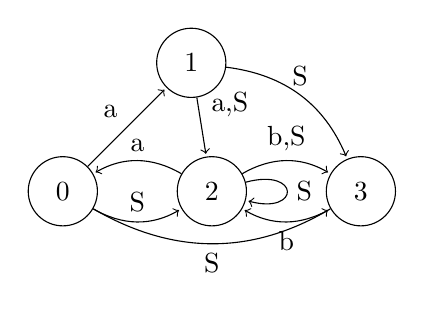
\begin{tikzpicture}[shorten >=1pt,auto]
        \node[state] (q_0)                      {$0$};
        \node[state] (q_1) [above right=of q_0] {$1$};
        \node[state] (q_2) [right=of q_0]       {$2$};
        \node[state] (q_3) [right=of q_2]       {$3$};
          \path[->]
            (q_0) edge  node {a} (q_1)
            (q_1) edge  node {a,S} (q_2)
            (q_2) edge[bend right, above]  node {a} (q_0)
            (q_2) edge[loop right]  node {S} (q_2)
            (q_1) edge[bend left, above]  node {S} (q_3)
            (q_0) edge[bend right, above]  node {S} (q_2)
            (q_2) edge[bend left, above]  node {b,S} (q_3)
            (q_0) edge[bend right, below]  node {S} (q_3)
            (q_3) edge[bend left, below]  node {b} (q_2);
    \end{tikzpicture}
    \end{center}{}
    \caption{The result graph $\mathcal{G}$ for example query}
    \label{example:result}
\end{figure}{}
\section{Evaluation}

This section describes the methodology and answers the following research questions.

\begin{enumerate}
    \item Does fusion via distillation give any benefits at the software and hardware levels?
    \item What are the properties of the generated hardware?
    \item Does the generated hardware outperform software implementations?
\end{enumerate}

\subsection{Methodology}

Our focus is on creating a basis for future research and experiments, thus we make our experiments as much reproducible as possible\footnote{\url{https://github.com/sedwards-lab/fhw/tree/sparse-linear-algebra-distillation/examples/QTreeBenchmarks/diploma/verilog-bool-no-nnz-inlined} (online; accessed:
2022-06-07) Here one could find all the results. For each benchmark all statistics are specified: matrix names, their sizes, collected metrics for both hardware and software benchmarks.}. We benchmarked the following list of chained functions. The choice is prompted by the current state of the distiller: at the moment, it does not successfully distill matrix multiplication. However, the functions are still practical enough, for example, chained addition could be seen in Luby's maximal independent set algorithm and clearly describe the applicability of the proposed approach.

\begin{itemize}
    \item \mintinline{Haskell}{mAdd (==False) (||) (mAdd (==False) (||) m1 m2) m3}
    \item \mintinline{Haskell}{mask (mAdd (== False) (||) m2 m3) (m1)}
    \item \mintinline{Haskell}{map (==Zero) (to_nat) (mAdd (==False) (||) m1 m2}
    \item \mintinline{Haskell}{map (==Zero) (to_nat) (kron (==False) (&&) m1 m2}
\end{itemize}

Above, \mintinline{Haskell}{Zero} and \texttt{to\_nat} are corresponding definitions for Peano arithmetics, since the \texttt{.pot} language does not have any primitives. For the same reason, we operated with boolean matrices. Such functions could be abstracted with free variables and then instantiated in the emitted Haskell code. However, to get maximum from distillation, we provided all the information about the functions. 

For these functions, we compared the execution time of distilled and not distilled hardware generated circuits, execution time of original and distilled Haskell code and reference \textit{Suite Sparse}\footnote{\url{https://github.com/DrTimothyAldenDavis/GraphBLAS} (online; accessed:
2022-06-07), Suite Sparse library sources.}\textsuperscript{,}\footnote{The library also uses different variations of coordinate formats (opaque to the user) and not a quadtree representation.} variants of these functions in C\texttt{++}. Note that SuiteSparse does not support recursive data types, thus only the first two function chains were implemented in SuiteSparse (since Peano number is essentially a linked list). We did not replace Peano numbers with integers, so our experiments could be interpreted easier. For hardware experiments we collected execution time and the number of memory writes and reads, to access how well fusion is performed. For software experiments we only measured the execution time. Also note that we measured only the time, required to execute the lines above, not including any IO, required to get and evaluate function arguments. But in hardware benchmarks we measured the time required to pass arguments into the circuit's memory, because such IO is inevitable. It is tricky to make such measures in Haskell due to laziness, thus the programs were compiled with \texttt{--fno-full-laziness} to turn off memoization. Also all the arguments were forced to normal form via \texttt{force} and \texttt{evaluate}. Haskell programs were compiled\footnote{GHC 8.10.4.} with \texttt{-O2 --fno-full-laziness} and Suite Sparse was compiled with default flags and linked as a shared library to C\texttt{++} code.

We took matrices from SuiteSparse matrix collection with sizes ranging from \texttt{64x64} to \texttt{512x512}. We limited ourselves with such sizes due to the fact that this is the maximum sizes that fit into \texttt{bram} with $2^{16}$ address space. Such number of \texttt{bram} blocks is available only on really expensive FPGA boards, thus in practice sizes would be smaller to achieve better utilization. Once again, it models the situation when data fits into the cache, since \texttt{bram} in our circuits will operate as a cache in real application.

\subsection{Experiments}

Table~\ref{tab:bench_results} shows the results of all execution time benchmarks. To evaluate execution time for hardware simulation, implementation stage was performed to assess the maximum frequency of FPGA device used for synthesis and implementation, and the number of execution cycles was multiplied by the number of nanoseconds a clock cycle takes. The frequencies were equal within the same benchamark set, i.e., frequency was not affected by distillation. We used \texttt{xcu250figd2104-2L} device\footnote{\url{https://www.xilinx.com/products/boards-and-kits/alveo/u250.html}  (online; accessed:
2022-06-07)} for synthesis and implementation stages. It is not really a casual and affordable chip, but it contains enough \texttt{bram} for our evaluation to see scalability. In the table a median across several benchmarks is shown. 

As it could be seen, distillation steadily increases performance: up to 2x speedup for hardware simulation and up to 3x for software benchmarks. The results are maintained within the borders of the corresponding confidence interval and the borders are not shown for brevity. Hardware speedup is lower due to the different execution semantics, dataflow is not reduction-based and distillation is a reduction-based transformation. Note that generated hardware appears to be less performant than both Haskell and C\texttt{++}, which a bit contradicts the results from~\cite{oldfhw}. For hardware benchmarks \texttt{time (IO)} shows the execution time including the time needed to transfer the data though the arguments, \texttt{time (no IO)} does not include it in its turn. It could be seen that not all the benchmarks are computationally extensive enough to cover memory transferring costs, but for more complex examples the ratio would be better. Since we basically transfer the matrices node by node from a file in the testbench, we have probably the lowest possible latency, and in practice it would be higher if reading from DDR, however the bandwidth could be increased. Noticeably, running times for \texttt{mMaskAdd} for C\texttt{++} and distilled Haskell are similar, which shows that fusion really provides some extra performance: SuiteSparse at the moment does not implement any fusion.

Table~\ref{tab:mem_results} summarizes the ratios between distilled and not distilled hardware circuits memory reads and writes. Since in general case distillation removes extra pattern matching, essentially it saves memory reads and writes. The eventual number of memory reads and writes is implementation dependent, thus the table shows what share of speedup is prompted by saving memory operations. Distillation successfully reduces the number of memory accesses, about 15\% on average. \texttt{mMapKron} has a bit higher ratio due to the fact that \texttt{Nat} numbers require additional memory accesses, since the type is recursive. It could also be seen that a major part of speedups is attributed to saved memory accesses. 

Finally, table~\ref{tab:resource_util} shows device resources utilization ratios between distilled and not distilled hardware circuits and frequencies. Columns are device primitives: registers, lookup tables, \texttt{bram} blocks or multiplexers. Utilization for both types of circuits is below 1\% of available resources on the device, except for the memory. Memory blocks utilization is about 30\% (since we choose larger \texttt{brams} to store larger matrices). Apart from that, distilled circuits could have both higher and lower utilization. Since the hardware generation is primarily syntax-directed it follows from the distilled program structure. For example, distillation might glue two recursive functions into one (in that case, memory utilization would be lower, because each cluster of mutually recursive functions possesses its own heap) or make more recursive functions than in the original program. The frequencies are the same, however, they possibly could be made better with more intelligent buffer allocation.

\subsection{Discussion}
Answering the research questions above.

\begin{enumerate}
    \item Fusion gives significant benefits, however at the hardware level the benefits are a bit smaller since hardware semantics is not reduction based. The benefits at the hardware level are mostly determined by the reduced number of memory accesses (each access takes 2 clock cycles). Notably, distilled Haskell implementation of \texttt{mMaskAdd} has similar performance with C\texttt{++}. 
    \item Device utilization is low, but such circuits could be copied on the same device to provide better utilization and higher parallelism. Resource utilization might be both better and worse after distillation, depending on the transformed program itself since translation is syntax-directed. Frequency could be increased by more intelligent buffering strategy.
    \item Although we use low-latency design with \texttt{bram}s that take 2 clock cycles per request and transfer matrices from files, which does not have any latency in simulation, we get slower execution time than Haskell and C\texttt{++} counterparts. It could be partly due to excessive buffering performed by FHW at the moment. Also there is no pipelining for recursive calls, i.e. only one set
of function argument tokens are allowed to enter a tail-recursive function call until a result is finally generated. Further CPS transformation hinders parallelization, which could be made more explicit with SSA. Some other optimizations exist that may significantly influence the performance. Also, since device utilization is about 1\%, such circuits could be copied on one device and provide more parallelism. A more detailed discussion could be found at~\cite{Edwards2019FHWP}.
\end{enumerate}

Distillation clearly showed its applicability to optimization of sparse linear algebra routines and notably it still could be combined with other techniques, like rewrite rules to achieve better results. High-level synthesis has a room for improvements by increasing pipelining, parallelism and frequency and the generated hardware could be improved from usability perspective: a support for arbitrary sized matrices is desirable. Thus we will focus on these directions. Probably a better solution would be to embed \texttt{.pot} language into e.g. Haskell to leverage its type system (to be able to use some rewrite rules as well), and add support for primitive types and parallel primitives to be able to conduct a more scalable comparison with SuiteSparse (since SuiteSparse is multithreaded). For such embedding different execution models could be implemented, including hardware synthesis, for which SSA form of GRIN looks promising, as well as extra optimizations shipped with GRIN. For hardware synthesis, an interesting direction is achieving predictable results in hardware from certain modifications in software. This property partly holds for the current approach, since the translation is syntax- directed. More information on this could be found at~\cite{predict}.

\pagebreak

\begin{table}[t]
\scriptsize
\centering
\caption*{mAddAdd}
\begin{tabular}{|c|c|c|c|c|c|c|c|c|c|} 
\hline
\rowcolor{LightBlue}
\multicolumn{3}{|c|}{Matrices dimensions} & Haskell & Haskell (distilled) & \multicolumn{2}{c|}{FHW} & \multicolumn{2}{c|}{FHW (distilled)} & {C\texttt{++}}\\
% \rowcolor{LightBlue}
\hline
m1 & m2 & m3 & time & time & time (no IO) & time (IO) & time (no IO) & time (IO) & time \\ 
\hline
64 & 64 & 64 & 29 us & 20 us & 76 us & 170 us & 64 us & 158 us & 14 us\\ 
128 & 128 & 128 & 94 & 79 & 146 & 476 & 134 & 469 & 30 \\
256 & 256 & 256 & 123 & 103 & 202 &  681 & 168 & 662 & 44\\
512 & 512 & 512 & 219 & 143 & 474 & 1192 & 375 & 1093 & 49\\
\hline
\end{tabular}

\caption*{mMaskAdd}
\begin{tabular}{|c|c|c|c|c|c|c|c|c|c|} 
\hline
\rowcolor{LightBlue}
\multicolumn{3}{|c|}{Matrices dimensions} & Haskell & Haskell (distilled) & \multicolumn{2}{c|}{FHW} & \multicolumn{2}{c|}{FHW (distilled)} & {C\texttt{++}}\\
% \rowcolor{LightBlue}
\hline
m1 & m2 & m3 & time & time & time (no IO) & time (IO) & time (no IO) & time (IO) & time \\ 
\hline
64 & 64 & 64 & 10 us & 7 us & 64 us & 133 us & 46 us & 111 us & 18 us\\ 
128 & 128 & 128 & 38 & 30 & 118 & 322 & 75 & 292 & 33 \\
256 & 256 & 256 & 48 & 42 & 168 &  498 & 104 & 456 & 46\\
512 & 512 & 512 & 126 & 76 & 400 & 762 & 300 & 729 & 65\\
\hline
\end{tabular}

\caption*{mMapAdd}
\begin{tabular}{|c|c|c|c|c|c|c|c|c|c|} 
\hline
\rowcolor{LightBlue}
\multicolumn{3}{|c|}{Matrices dimensions} & Haskell & Haskell (distilled) & \multicolumn{2}{c|}{FHW} & \multicolumn{2}{c|}{FHW (distilled)} & {C\texttt{++}}\\
% \rowcolor{LightBlue}
\hline
m1 & m2 & m3 & time & time & time (no IO) & time (IO) & time (no IO) & time (IO) & time \\ 
\hline
64 & 64 & --- & 45 us & 37 us & 189 us & 253 us & 137 us & 202 us & ---\\ 
128 & 128 & --- & 162 & 105 & 524 & 685 & 397 & 579 & --- \\
256 & 256 & --- & 312 & 216 & 1047 &  1360 & 680 & 986 & ---\\
512 & 512 & --- & 436 & 273 & 1346 & 1776 & 900 & 1330 & ---\\
\hline
\end{tabular}

\caption*{mMapKron}
\begin{tabular}{|c|c|c|c|c|c|c|c|c|c|} 
\hline
\rowcolor{LightBlue}
\multicolumn{3}{|c|}{Matrices dimensions} & Haskell & Haskell (distilled) & \multicolumn{2}{c|}{FHW} & \multicolumn{2}{c|}{FHW (distilled)} & {C\texttt{++}}\\
% \rowcolor{LightBlue}
\hline
m1 & m2 & m3 & time & time & time (no IO) & time (IO) & time (no IO) & time (IO) & time \\ 
\hline
2 & 64 & --- & 64 us & 36 us & 212 us & 242 us & 94 us & 125 us & ---\\ 
2 & 128 & --- & 137 & 68 & 434 & 502 & 199 & 266 & --- \\
2 & 256 & --- & 364 & 126 & 1004 &  1188 & 449 & 636 & ---\\
4 & 128 & --- & 302 & 94 & 694 & 763 & 330 & 401 & ---\\
\hline
\end{tabular}



\caption{Execution time}
\label{tab:bench_results}

\end{table}
\begin{table}[h]
\scriptsize
\begin{minipage}{0.45\linewidth}
\centering
\caption*{mAddAdd}
\begin{tabular}{|c|c|c|c|c|c|c|} 
\hline
\rowcolor{LightBlue}
\multicolumn{3}{|c|}{Matrices dimensions} & \multicolumn{2}{c|}{Ratio ($\frac{FHW}{FHW_{distilled}}$)}\\
% \rowcolor{LightBlue}
\hline
m1 & m2 & m3 & writes & reads\\ 
\hline
64 & 64 & 64 & 1.10 & 1.15\\ 
128 & 128 & 128 & 1.02 & 1.05\\
256 & 256 & 256 & 1.03 & 1.06\\
512 & 512 & 512 & 1.10 & 1.16\\
\hline
\end{tabular}
\end{minipage}
\begin{minipage}{0.45\linewidth}
\centering
\caption*{mMaskAdd}
\begin{tabular}{|c|c|c|c|c|c|c|} 
\hline
\rowcolor{LightBlue}
\multicolumn{3}{|c|}{Matrices dimensions} & \multicolumn{2}{c|}{Ratio ($\frac{FHW}{FHW_{distilled}}$)}\\
% \rowcolor{LightBlue}
\hline
m1 & m2 & m3 & writes & reads\\ 
\hline
64 & 64 & 64 & 1.13 & 1.26\\ 
128 & 128 & 128 & 1.06 & 1.11\\
256 & 256 & 256 & 1.08 & 1.09\\
512 & 512 & 512 & 1.10 & 1.16\\
\hline
\end{tabular}
\end{minipage}
\begin{minipage}{0.45\linewidth}
\centering
\caption*{mMapAdd}
\begin{tabular}{|c|c|c|c|c|c|c|} 
\hline
\rowcolor{LightBlue}
\multicolumn{3}{|c|}{Matrices dimensions} & \multicolumn{2}{c|}{Ratio ($\frac{FHW}{FHW_{distilled}}$)}\\
% \rowcolor{LightBlue}
\hline
m1 & m2 & m3 & writes & reads\\ 
\hline
64 & 64 & --- & 1.10 & 1.21\\ 
128 & 128 & --- & 1.07 & 1.14\\
256 & 256 & --- & 1.07 & 1.19\\
512 & 512 & --- & 1.10 & 1.21\\
\hline
\end{tabular}
\end{minipage}
\hfill
\begin{minipage}{0.45\linewidth}
\centering
\caption*{mMapKron}
\begin{tabular}{|c|c|c|c|c|c|c|} 
\hline
\rowcolor{LightBlue}
\multicolumn{3}{|c|}{Matrices dimensions} & \multicolumn{2}{c|}{Ratio ($\frac{FHW}{FHW_{distilled}}$)}\\
% \rowcolor{LightBlue}
\hline
m1 & m2 & m3 & writes & reads\\ 
\hline
2 & 64 & --- & 1.71 & 1.88\\ 
2 & 128 & --- & 1.72 & 1.87\\
2 & 256 & --- & 1.65 & 1.83\\
4 & 128 & --- & 1.81 & 1.91\\
\hline
\end{tabular}
\end{minipage}

\caption{Memory accesses}
\label{tab:mem_results}
\end{table}

\begin{table}[h]
\scriptsize
\centering
\begin{tabular}{|l|c|c|c|c|c|c|c|c|c|} 
\hline
\rowcolor{LightBlue}

{Benchmark} & \multicolumn{8}{c|}{Ratio (${\frac{FHW}{FHW_{distilled}}}$)} & {Frequency}\\
\hline
{} & FDRE & LUT3 & LUT6 & LUT5 & LUT4 & LUT2 & RAMB36E2 & MUXF7 & {} \\
% \rowcolor{LightBlue}
\hline
mAddAdd & 0.3 & 0.3 & 0.3 & 0.5 & 0.3 & 0.3 & 0.5 & 0.5 & 200 MHz\\ 
mMaskAdd & 0.5 & 0.5 & 0.7 & 0.4 & 0.7 & 0.5 & 0.7 & 0.6 & 200 MHz\\
mMapAdd & 1 & 0.9 & 0.9 & 1.2 & 1 & 1.1 & 1.1 & 1.2 & 200 MHz\\
mMapKron & 1.5 & 1.5 & 1.3 & 2 & 2 & 1.8 & 1.4 & 1.7 & 200 MHz\\
\hline
\end{tabular}
\caption{Resource utilization}
\label{tab:resource_util}
\end{table}
\pagebreak

\section{Conclusion and Future Work}

We present !!!

Our evaluation shows that !!!

First direction for future research is a more detailed CFPQ algorithms investigation.
We should do More evaluation on sparse matrices on GPGPUs.

Also it is nesessary to implement and evaluate solutions for graphs which is not fit in RAM.
There is a set of technics for huge matrices multiplication.
Is it possible to dopt it for CFPQ

Another direcion is a dataset improvement.
More data.
More grammars/queries.


%
% ---- Bibliography ----
%
% BibTeX users should specify bibliography style 'splncs04'.
% References will then be sorted and formatted in the correct style.
%
 \bibliographystyle{splncs04}
 \bibliography{tensor_product_cfpq}
\end{document}
